\documentclass[12pt, a4paper, oneside, romanian]{teza-upb}
\setcounter{secnumdepth}{3}
\setcounter{tocdepth}{3}
\usepackage{babel}
\usepackage{graphicx}
\usepackage{float}
\usepackage[
  bookmarksnumbered,
  bookmarks,
  bookmarksopen=true,
  pdftitle={Dizertatie},
  linktocpage]{hyperref}
\singlespacing
\begin{document}
\begin{titlepage}
	\centering
	
\includegraphics[width=0.15\textwidth]{img/UPB-logo.png}\par\vspace{1cm}
	{\scshape\LARGE Facultatea de Electronică, Telecomunicații și Tehnologia Informației \par}
	\vspace{1cm}
	{\huge Sesiunea de comunicări sțiințifice\par}
	{\large 2016 \par}
	\vspace{1cm}
	{\huge\bfseries Arhitecturi pentru sisteme auto-scalabile: microservicii\par}
	\vspace{2cm}
	{\Large\bfseries Andrei Mihăescu\par}
	\vspace{2cm}
	{\Large\bfseries Conducători științifici: \par}
	{\Large Conf. dr. ing. Eduard-Cristian POPOVICI \par}
	{\Large Ș.l. dr. ing. Radu BADEA\par}
% Bottom of the page
\end{titlepage}
\tableofcontents
\listoffigures
\newpage

\chapter{Motivație}

Datorită avansurilor tehnologice uriașe în domeniul informaticii și al telecomunicațiilor astăzi, mai mult ca niciodată, o foarte mare parte a activităților coditiene (fie ele profesionale sau personale) sunt stâns legate de domeniul virtual. Revoluția digitală a schimbat complet modul în care folosim sistemele informatice, care acum stau la baza foarte multor afaceri din toate domeniile (plecând de la cel bancar și terminând cu cel agricol) în proporție de 24\% cu previziuni ca această cifra să se dubleze până în 2020 - \textit{"Forrester Research - The State of Digital Business, 2015 to 2020"}.

Această expansiune a pus o presiune enormă asupră inginerilor din domeniul informatic, care se confruntă cu o adevărată provocare pentru a crea sisteme robuste capabile să satisfacă această nevoie crescândă. Pornind de la această nevoie, conceptul de aplicație de tip "enterprise" a luat naștere. O astfel de aplicație trebuie să răspundă anumitor standarde și cerințe pentru a putea asigura buna funcționare a unei afaceri:
\begin{itemize}
 \item \textbf{flexibilitate} - o aplicație bine gândită trebuiă să permită modificări, ce apar ca urmarea a evoluției domeniului în care este folosită; aceastea trebuie ușor implementate, pentru a crea valoare pentru utilizatori.
 \item \textbf{robustețe} - în proiectarea unei aplicații trebuie luate în calcul cât mai multe cazuri în care aceasta ar putea fi exploatată și compromisă, creând astfel întreruperi în funizarea serviciilor.
 \item \textbf{scalabilitate} - având in vedere dorința fiecărei afaceri de a prospera și a crește este de așteptat ca și aplicațiile folosite să se poată adapta la volume din ce în ce mai mari de procesări. 
 \item \textbf{securitate} - dat fiind faptul că o aplicație poate deveni principala sursă de venit din cadrul unei companii este nevoie ca aceasta să respecte cel mai înalte standarde de securitate astfel încât datele utilizatorilor să fie bine protejate. 
\end{itemize}

Pentru a răspunde tuturor acestor nevoii, un sistem informatic trebuie să fie slab cuplat (eng. \textit{loosely-coupled}), pentru a asigura flexibilitate, să aibă mecanisme ce asigură redundanța, pentru robustețe, să aibă un grad mare de modularizare pentru a fi scalabil și să implementeze principiul eng. \textit{AAA - Authentication, Authorization \& Accounting} pentru a fi sigur.


\chapter{Aplicații monolit}

Aplicațiile \textbf{monolit} reprezintă modul tradițional de dezvoltarea a unei aplicații, fie ea chiar și de tip enteprise. În cadrul aplicațiilor monolit toată funcționalitatea este dezvoltată în cadrul unui artefact care este livrat la final și trimis în producție. Acest model prezintă o serie de avantaje și dezavantaje. 

Printre primele avantaje ale acest tip de aplicație se numără faptul că este ușor de dezvoltat; din punct de vedere arhitectural nu implică eforturi mari. Totul este dezvoltat ca un singur bloc a cărui componente pot fi organizate pe module, însă sunt reunite și livrate sub forma unui singur produs final. În mod tipic o astfel de aplicație va rula pe unul sau mai multe servere. Fiecare dintre acestea fiind identic toate componentele din cadrul aplicație vor comunica între ele la nivel de proces, fără a implica vreun fel de comunicare cu exteriul, exceptând prin intermediul punctelor terminale (\textit{eng. end point}) special construite. Acest tip de aplicație prezintă un grad relativ scăzut de complexitate, aceasta din punct de vedere arhitectural, deoarece complexitatea logici de business nu este corelată cu arhitectura aplicației. Mentenanța unei astfel de aplicații este facilă, întreg codul situându-se într-un singur loc, procesul de depanare se poate desfăsura ușor. 

În ciuda acestor avantaje care ar putea înclină balanța în favoarea aplicațiilor monolit,ele prezintă o serie de dezavantaje care îngreunează procesul de creare de valoare prin implementarea nevoilor unei afaceri. Faptul că toate componentele sunt în cadrul unui singur artefact determină un nivel înalt de cuplare între acestea - \textit{eng. tightly coupled} - ceea ce duce la o scădere a flexibilității și deci o reducere a ritmului de implementare a schimbărilor. Legat de acest fapt este randamentul slab în ceea ce privește scalabilitatea. Aplicația nu poate scala decât cu o granularitate de o instanță, nu de un modul al său de care poate fi nevoie. Astfel spus, pentru a îmbunătații performanța unui modul toată aplicație trebuie instalată pentru un alt server. Un dezavantaj, ar fi legat de modul de instalare a aplicațiilor pe diverse medii (dezvoltare, testare sau producție). Adesea o nouă instalare (\textit{eng. deploy}) vizează o singură componentă, însă pentru a livra schimbarea toată aplicația trebuie recompilată și instalată.

Deși avantajele acestor aplicații nu sunt de neglijat, ele prezintă dezavantaje care le fac să nu mai fie relevante în contextul actual al tendințelor, care orientate pe flexibilitate și pe livrarea în producție cât mai rapidă a produselor informatice. 

\chapter{Aplicații bazate pe microservicii}

Aplicațiile bazate pe microservicii fac parte dintr-o categorie mai largă de aplicații care sunt înscriu în capitolul aplicațiilor orientate pe servicii (\textit{eng. SOA - Service Oriented Architecture}). Caracteristicile arhitecturii SOA sunt:
\begin{itemize}
 \item Serviciile sunt autonome. Fiecare serviciu este menținut, dezvoltat, instalat și versionat în mod independent.
 \item Serviciile pot fi distribuite. Serviciile pot fi localizate oriunde pe rețea, local sau la distanță, atât timp cat rețeaua dispune de protocoalele necesare de comunicare.
 \item Serviciile sunt slab cuplate. Fiecare serviciu este independent față de celălalte și poate fi înlocuit și actualizat fără a întrerupe celălalte aplicații care îl folosesc atât timp cât interfețele sunt compatibile.
 \item Serviciile împart schema și contractul, nu clasa. Serviciile partajează contracte și scheme atunci când comunică, și nu clase interne.
\end{itemize}


Plecând de la aceste caracteristici ideea microserviciilor duce mai departe distribuirea și slaba cuplare a serviciilor, astfel că dezvoltarea unuei aplicații este realizată ca o suită de mici servicii, fiecare rulând un proces independent și comunicând prin mecanisme simple, adesea resurse expuse prin API-uri via HTTP. Pe lângă faptul ca serviciile pot fi instalate și scalate în mod independent, fiecare crează o limită fermă a modulului, permițând chiar și folosirea limbajelor de programare diferite, acestea putând fii gestionate de echipe diferite.

\section{Caracteristici}

Aplicațiile bazate pe microservicii folosesc librării, însă modalitatea principală prin care se face componentizarea reprezintă împărțirea pe servicii. Definim \textbf{bibliotecile} ca fiind componente ce funcționează împreună în cadrul unui program și deci au memorie comună, în vreme ce \textbf{serviciile} sunt componente ce rulează în cadrul unor procese diferite și care comunică prin mecanisme cum ar fi cereri de tip web sau \textbf{RPC} (Remote Procedure Call).

Unul din motivele pentru folosirea serviciilor ca și componente (mai degrabă decât biblioteci) este faptul că serviciile pot fi instalate în mod independent. În cazul unei aplicații constituită din mai multe biblioteci aparținând unei singure instanțe, o schimbare a oricărei componente ar rezulta în reinstalarea întregii aplicații. Dacă însă aplicația este descompusă în mai multe servicii, este de așteptat ca modificările la nivel de serviciu să nu necesite decât reinstalări alei acestuia. Acest lucru nu este universal valabil, unele modificări ar putea impacta interfețe ale mai multor serviciilor necesitând o sincronizarea la nivelul mai multor servicii, însă ținta unei arhitecturi bazate pe microservicii este minimizarea acestui impact prin precizarea funcționalităților in cadrul contractelor.

Când se dorește împărțirea unei aplicații în componente, adesea divizarea echipei se face în funcție de nivelul tehnologic, astfel formându-se echipe responsabile pentru interfața grafică, logica de server și baza de date. Când acestă împărțire este realizată, chiar și cele mai simple schimbări pot duce la proiecte realizate de mai multe echipe ceea ce consumă timp și bani.

Abordarea separării componentelor diferă în cadrul microserviciilor, aceasta făcându-se ținând cont nevoile de business. Astfel de servicii preiau intreagă stivă tehnologică ce include interfața grafică, stocarea și orice colaborare externă. În consecință echipele sunt trans-funcționale, cuprinzând o plajă largă de cunoștințe necesare pentru dezvoltare: proiectarea interfeței grafice, baze de date și project management. 

Pentru construirea unor structuri de comunicare între diferite procese există multe procese și abordări care se concentrează pe implementarea inteligenței în mecanismul de comunicare în sine. Un exemplu foarte bun este Entreprise Service Bus (\textbf{ESB}), aceste mecanisme oferind capacități complexe pentru rutarea mesajelor și aplicarea regulilor de business.

Microserviciile implică o altă abordare: puncte terminale inteligente și bus-uri simple (eng. "smart endpoints and dumb pipes"). Aplicațiile ce urmează aceste principii tind să fie cât mai decuplate, primind o cerere, aplicând logica adecvată și producând un răspuns. Acești pași sunt corelați folosind protocoale simple de tip REST mai degrabă decât cele complexe precum WS-Choreography, BPEL sau orchestrare prin intermediul unuei unelte centrale. 

Cele mai folosite două protocoale sunt HTTP cerere-răspuns folosind API-uri pentru accesarea resurselor și mecanisme simple de trimiterea mesajelor. Echipele care lucrează cu microservicii folosesc principiile și protocoalele pe baza caror a fost construit și web-ul. 

Al doilea mecanism folosit este cel al mesajelor transmise prin intermediul unui bus simplu. Infrastructura aleasă este adesea simplă (nu are decât rolul de a ruta mesajele) - implementări simple precum RabbitMQ sau ZeroMQ nu fac mai mult decât să pună la dispoziție un canal de comunicare asincron - inteligența rămânând în punctele terminale ce produc și consumă mesajele.

Datorită numărului mare de componente, microserviciile se bazează pe automtizarea infrastructurii pentru livrarea componentelor în mod repetabil în diversele medii. 

Tehnicile pentru automatizarea infrastructurii au evoluat foarte mult în ultimii ani - evoluția clodului și a furnizorilor de infrastructură ca serviciu (\textit{eng. Infrastructure as a Service}). Acest lucru a redus foarte mult complexitatea operațională pentru gestionarea microserviciilor. 

Multe dintre produsele și sistemele folosind microservicii sunt construite de echipe cu experiență în Continous Delivery și predecesorul său, Continous Integration. Echipele ce construiesc astfel aplicațiile folosesc în mod extensiv tehnici de automatizare a infrastructurii. Acest lucru, denumit în literatura de specialitate \textbf{"pipeline"}, este ilustrat mai jos:

\begin{figure}[ht]
\centering
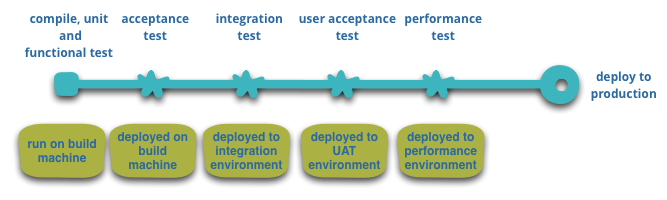
\includegraphics[scale=0.6]{img/basic-pipeline.png}
\caption{Pipeline}
\label{fig:arhi_componente}
\end{figure}

Un \textbf{"pipeline"} reprezintă o înlățuire de procese care trebuie urmate de fiecare dată când se dorește instalarea aplicației pe un mediu diferit. Aceste procese includ, compilarea aplicație, rularea testelor unitare și a celor de integrare, împachetarea ei și a tuturor resurselor necesare și eventual instalarea acesteia pe serverul dorit.

Câteva aspecte-cheie ale procesului de livrare continuă (e.g. Continous Delivery) sunt: încrederea cât mai mare în faptul calitatea software-ului dată de o suită foarte mare de teste automate; trecerea dintr-un mediu în altul în cadrul pipeline-ului înseamnă instalarea automată pe fiecare nou mediu. 

O aplicație monolit va fi compilată, testată și trecută prin aceste medii fără prea multe probleme. S-a constatat că investirea în automatizarea procesului de instalarea a unei aplicații în producție crește încrederea echipelor de a livra mult mai des pe acest mediu. Unul din obiectivele livrării continue este banalizarea procesului de instalare, astfel încât nu contează că se livrează una sau mai multe aplicații, lucrurile rămân la fel de simple. 

O altă aria în care se observă folosirea extensivă a automatizării infrastrucurii este administrarea microserviciilor în producție. În contrast cu afirmația precedentă legată de banalizarea instalării aplicațiilor în producție, peisajul operațional este complet diferit. 

\begin{figure}[ht]
\centering
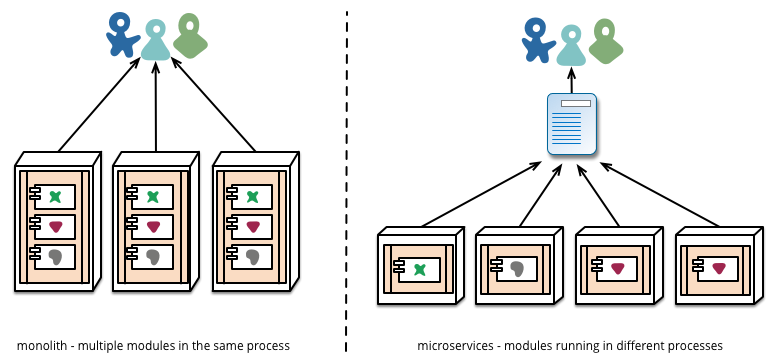
\includegraphics[scale=0.6]{img/micro-deployment.png}
\caption{Instalarea modulelor diferă}
\label{fig:arhi_componente}
\end{figure}

\section{Avatanje și dezavantaje ale microserviciilor}
\subsection{Avatanje}
Microserviciile prezintă un număr important de avantaje. În primul rând, rezolvă problema complexității, prin descompunerea a ceea ce altfel ar fi fost un aplicație monolit foarte mare într-un set de servicii. Fiecare serviciu conține un set bine definit de funcționalități expuse folosind RPC sau un API. Prin aceasta se crează un grad de modularitate care în practică ar fi extrem de greu de obținut în cadrul unei aplicații monolitice. În consecință serviciile individuale sunt mult mai rapid de dezvoltat și mult mai simplu de înțeles și menținut. 

Această arhitectură permite fiecărui serviciu să fie dezvoltat în mod independent de către o altă echipă. Dezvoltatorii au posibilitatea de a alege orice tehnologie consideră optimă pentru îndeplinirea cerințelor, în condițiile în care reușesc să expună în mod corect API-ul stabilit. În plus, serviciile fiind relativ mici, devine fezabilă rescrierea unui serviciu vechi folosind technologie actuală. 

Fiecare microserviciu poate să fie instalat în mod independent. Dezvoltatorii nu mai au nevoie să coordoneze instalarea modificărilor care sunt specifice serviciului lor. Aceste modificări pot fi instalate imediat ce au fost testate. De exemplu, echipa responsabilă de interfața grafică poate să efectueaze rapid teste și să implementeaze schimbări. Această arhitectură face posibilă integrarea continuă. 

În ultimul rând, microserviciile permit fiecărui serviciu să fie scalat în mod individual. Pot fi instalate doar numărul necesar de instanțe pentru fiecare serviciu care satisface nevoile de capacitate și disponibilitate. În plus se poate folosi un suport fizic care să corespundă nevoilor serviciilor. De exemplu un serviciu de procesare a imaginilor, care solicită foarte mult procesorul, poate fi instalat pe o instanță EC2 Compute-Optimized în vreme ce o bază de date în memorie poate fii instalată pe o instanță EC2 Memory-Optimized.

\subsection{Dezavantaje}

Ca orice tehnologie, arhitectura microservicii prezintă dezavantaje. Un prim dezvantaj este complexitatea care rezultă din faptul ca o aplicație ce folosește microservicii este un sistem distribuit. Dezvoltatorii trebuie să aleagă și să implementeze sunt mecanism de comunicare inter-proces bazat fie pe mesaje fie pe RPC. În plus, trebuie să scrie cod care să se gestioneze situațiile în care furnizorul de serviciu este încet sau indisponibil. În vreme ce niciuna din aceste probleme nu este foarte complexă, este considerabil mai complexă decât o aplicație monolit un module comunică prin apeluri de proceduri la nivel de limbaj.   

O altă provocare a microserviciilor o reprezintă arhitectura distribuită a bazei de date. Tranzacțiile de business care modifică entități multiple sunt ceva comun. Acest tip de tranzacții sunt trivial de implementat în cadrul unei aplicații monolit deoarece există o singură bază de date. Într-o arhitectură bazată pe microservicii multiplele baze de date ale serviciilor trebuie actualizate. Folosirea unui sistem distribuit de tranzacții nu este în mod normal o opțiune, și nu doar datorită Teoremei CAP - denumită și Teorema lui Brewer, care afirmă că este imposibil ca un sistem informatic să ofere simultan constrângerile următoare: consistență, disponibilitate și toleranță parțială. Ele pur și simplu nu sunt suportate de sistemele de baze de date NoSQL și nici de brokerii de mesaje. Compromisul este folosirea unei abordări bazate pe consistență, care este mai problematică pentru dezvoltatori. 

Testarea microserviciilor este mult mai complexă. De exemplu, folosind o bibliotecă modernă precum Spring Boot este foarte simplu de scris o clasă de test care pornește o aplicație web monolitică și care îi testează API-ul. În contrast cu aceasta, un test similar pentru un serviciu ar necesita lansarea serviciului și a serviciilor de care depinde, sau simularea acestora. Încă odata, acestea nu sunt foarte complex de realizat însă este importantă estimarea efortului necesar pentru a face aceasta. 

Instalarea unei aplicații bazate pe microservicii este mult mai complexă. O aplicație monolit este pur și simplu instalată pe un set de servere identice ce se află în spatele unui load-balancer tradițional. Fiecare instanță este configurată cu locațiile serviciilor de infrastructură cum ar fi baza de date și broker-ul de mesaje. Pe de altă, o aplicație bazată pe microservicii este alcătuită dintr-un număr mare de servicii. Aceasta implică o complexitate crescută datorată nevoii de configurare, instalare, scalare și monitorizare a fiecăruia dintre servicii. În plus, este necesară implementarea unui mecanism de descoperire a serviciilor care să permite acestora să obțină adresa și portul altor servicii cu care ar avea nevoie să comunice. Modul tradițional de operare folosind tichete și operațiuni manuale nu scalează bine la acest nivel de complexitate. În consecință, instalarea cu succes a unei aplicații cu microservicii necesită un grad ridicat de control asupra procesului din partea dezvoltatorilor și un nivel înalt de automatizare. 

O soluție pentru obținerea automatizării este folosirea unui furnizor de servicii de tip "platforma ca serviciu" (eng. Platform as a Service - PaaS). Furnizorii de PaaS oferă dezvoltatorilor o modalitate simplă de instalare și administrare a microserviciilor. Acest îi izolează de probleme cum ar fi cumpărarea și configurarea de resurse IT. În același timp, specialiștii de sisteme și rețele care configurează PaaS se pot asigura că toate bunele practici au fost respectate. O altă soluție este dezvoltarea a prorpiului PaaS. Un punct de plecare ar putea fii o soluție de clustering, precum Mesos sau Kubernetes folosit impreună cu tehnologii precum Docker. 


\section{Construirea microserviciilor}

În vederea realizării unei aplicații folosind microservcii o modalitatea de interacțiune între aceasta și utilizatori trebuie aleasă. În cazul unei aplicații monolitice există doar un set de puncte terminale. Într-o arhitectura de tip microservicii, fiecare serviciu expune un set de funcționalități. Una din posibilele metode prin care se poate realiza comunicarea client aplicație este prin intermediul unui API gateway.

În cazul unei aplicații monolit, un client de mobil ar putea obține datele printr-un simplu apel REST către aplicație: \texttt{GET api.company.com/productdetails/productId}. Un load balancer ar ruta cererea către unul din cele N servere identice. Aplicația ar lansa diverse interogări ale bazei de date care ar întoarce un răspuns către client. 

Pe de altă parte, folosind microservicii, datele afișate pe pagină aparțin mai multor microservicii, caz în care o strategie de comunicare între clienți și servicii trebuie aleasă. 

În general o abordare mult mai bună decât comunicare directă între clienți și microservicii este folosirea a ceea ce se numește un API gateway. Un API gateway reprezintă un server care este punctul de intrare în sistem. Este similar cu șablonul "Facade" programarea orientată pe obiecte. API Gateway-ul încapsulează arhitectura internă a sistemului și expună un API care poate fi adaptat pentru fiecare client. S-ar mai putea ocupa și de alte funcții precum autentificare, monitorizare, load balancing, caching, administrarea și modelarea cererilor. 


\begin{figure}[ht]
\centering
\begin{minipage}{0.45\textwidth}
\centering
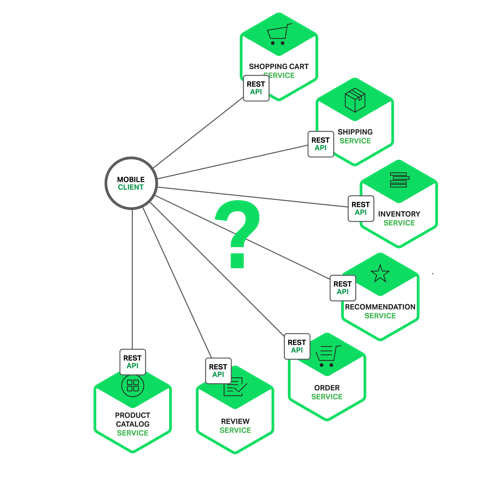
\includegraphics[scale=0.4]{img/Richardson-microservices-part2-2_microservices-client.png}
\caption{Folosirea unui API gateway}
\end{minipage}\hfill
\begin{minipage}{0.45\textwidth}
\centering
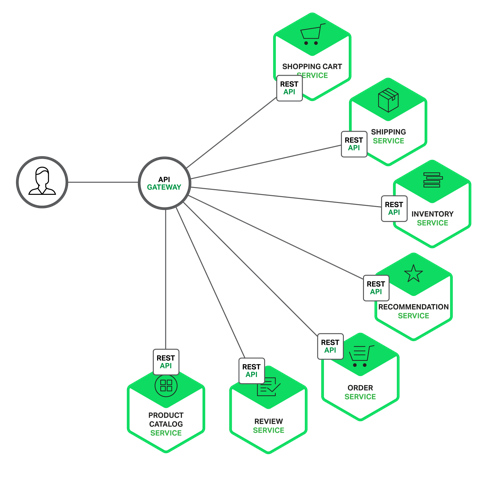
\includegraphics[scale=0.4]{img/Richardson-microservices-part2-3_api-gateway.png}
\caption{Diagramă a serviciilor}
\end{minipage}
\end{figure}

\section{Comunicarea inter-process}

Într-o aplicație monolit, componentele se invocă una pe cealaltă prin apeluri la de proceduri și metode la nivel de limbaj. Pe de alta parte, o aplicație bazată pe microservii este un sistem distribuit care rulează pe mai multe masini. Fiecare instanță a unui serviciu este un proces. În consecință, serviciile trebuie să interacționeze folosind un mecanism de comunicare inter-proces (\textit{IPC - eng. inter-process communication)}.

Interacțiunile intre procese pot fi de mai multe feluri, în funcție de mai multe criterii.  Un prim criteriu ar fi numărul de entități implicate: unu-la-unu, fiecare cerere a clientului este procesată de exact un singur serviciu, unu-la-mai-mulți, fiecare cerere este procesată de mai multe servicii. Al doilea criteriu de luat în calcul este caracterul sincron și astfel avem două categorii de interacțiuni: sincronă, clientul așteaptă răspunsul de la serviciul, timp în care blochează execuția altor operații și asincronă clientul nu blochează execuția și răspunsul, dacă există, nu trebuie trimis imediat.

Interacțiunile unu-la-unu pot fi de mai multe tipuri:

\begin{itemize}
 \item Cerere/răspuns - Un client lansează o cerere către un serviciu și asteaptă un răspuns. Clientul așteaptă răspunsul într-un timp rezonabil. Într-o aplicație care folosește fire de execuție, firul de execuție care lansează cererea s-ar putea chiar bloca în timp ce așteaptă. 
 \item Notificare - clientul trimite o cerere la un serviciu, însă un răspuns nu este așteptat.
 \item Cerere/răspuns asincron - un client trimite o cerere la un serviciu, care răspunde asincron. Clientul nu se blochează în timp ce așteaptă și este proiectat plecând de la presupunerea că răspunsul ar putea ajunge după o perioadă mai lungă de timp.
\end{itemize}
 
La fel ca cele unu-la-unu, și interacțiunile unu-la-mai-mulți pot fi de mai multe feluri:
publish/subscribe - un client publică un mesaj de notificare, care este consumat de zero sau mai multe servicii interesate sau publish/async responses - un client postează un mesaj de cerere și apoi așteaptă o perioadă de timp pentru răspunsurile de la serviciile interesate. 

Folosind aceste stiluri de interacțiune serviciile comunică între ele folosind API-uri (\textit{Application Programming Interface}). API-ul unui serviciu reprezintă contractul între serviciu și clienți. Indiferent de mecanismul IPC ales, este important ca API-ul serviciului să fie precis definit.

Ca orice componentă API-ul se va schimba de-a lungul existenței aplicației. Într-o aplicație monolit operațiune de schimbare este destul de simplă. Într-o aplicație bazată pe microservicii aceasta este mult mai dificilă, chiar daca toți consumatorii sunt în aceeași aplicație. În mod tipic, clienții nu pot fi forțați să schimbe versiune pe care o folosesc. Deasemenea, versiunile noi vor fi instalate incremental astfel încât cele noi și cele vechi vor rula în mod simultan. 
\newpage
\section{Identificarea serviciilor}

Pentru apelarea unui REST (Representational State Transfer) API este nevoie de lansarea unei cereri, care să includă locația de rețea a serverului (adresa IP și portul). În cazul unei aplicații monolit care rulează pe un server fizic, aceste informații sunt relativ statice. Ele ar putea fi citite de exemplu dintr-un fisier de configurare care este actualizate periodic. În schimb, într-o aplicație mondernă ce rulează în cloud si este bazată pe microservicii acest lucru este mult mai dificil de rezolvat după cum arată schema de mai jos:

\begin{figure}[ht]
\centering
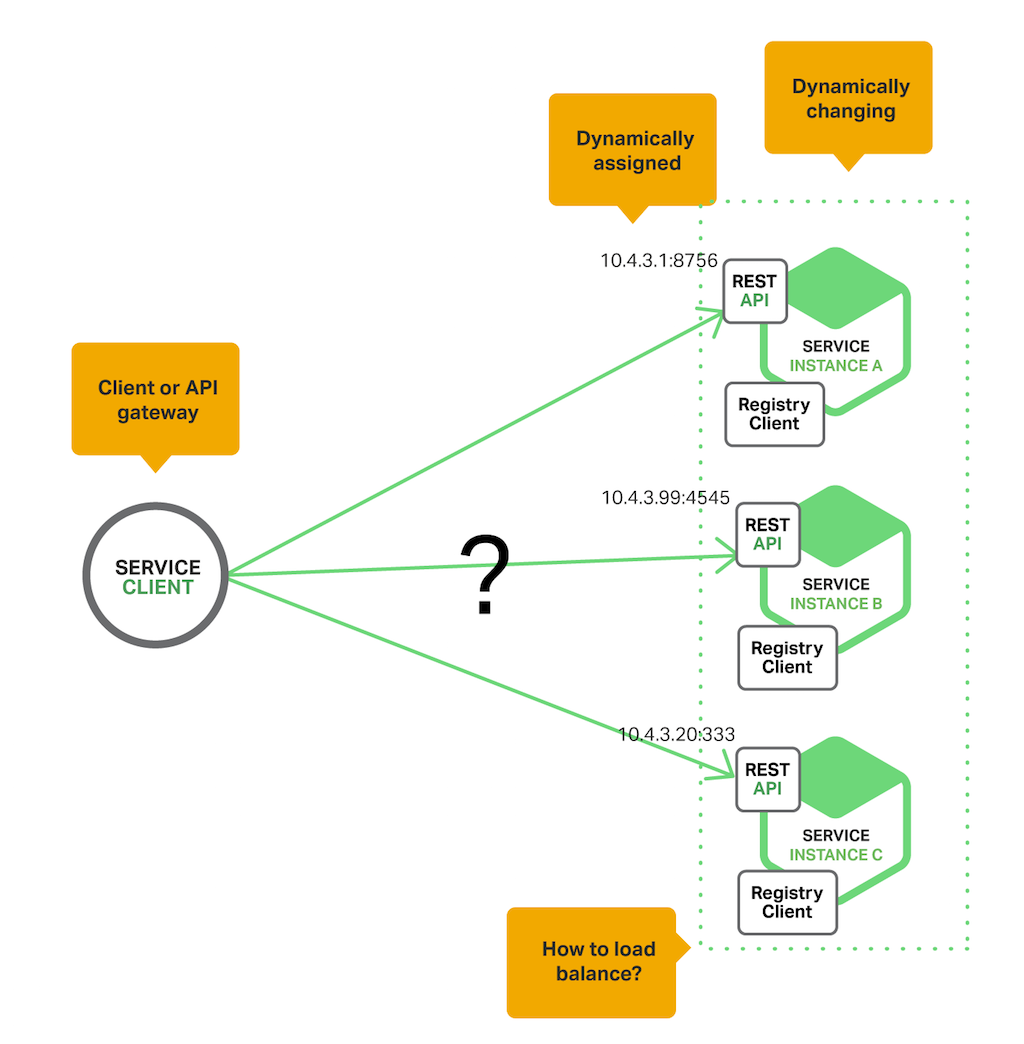
\includegraphics[scale=0.2]{img/Richardson-microservices-part4-1_difficult-service-discovery.png}
\caption{Identificarea serviciilor în cloud}
\label{fig:arhi_componente}
\end{figure}

Instanțelor serviciilor le sunt alocate în mod dinamic locații de rețea.  În plus, instațele se vor modifica în mod dinamic datorită auto-scalării, penelor și actualizărilor. În  consecintă codul client are nevoie de un mecanism mai elaborat de identificare a serviciilor. 

Există două categorii de șabloane: identificare pe partea de client (\textit{eng. client-side discovery}) și identificare pe partea de server (\textit{eng. server-side discovery}).

\subsection{Identificarea serviciilor de către client}

Atunci când descoperirea este realizată de către client, acesta este responsabil pentru determinare locațiilor de rețea ale instanțelor de serviciu și pentru a face balansare pe baza acestora. Clientul lansează o cerere către registrul de servicii (\textit{eng. sevice registry}), care este o bază de date a instanțelor de serviciu. Clientul apoi folosește un algoritm de balansare pentru a select unul dintre ele și pentru a lasa cererea propriu-zisă. 

Locația de rețea a unei instanțe de serviciu este înregistrată în registrul de serviciu atunci când este lansată. Este înlăturată atunci când instanța este oprită. Starea instanțelor serviciilor este actualizată period folosind un mecanism de tip puls (\textit{eng. heartbeat}).

\newpage

Principiul de funcționare al identificării serviciilor de către client funcționează conform schemei de mai jos:

\begin{figure}[ht]
\centering
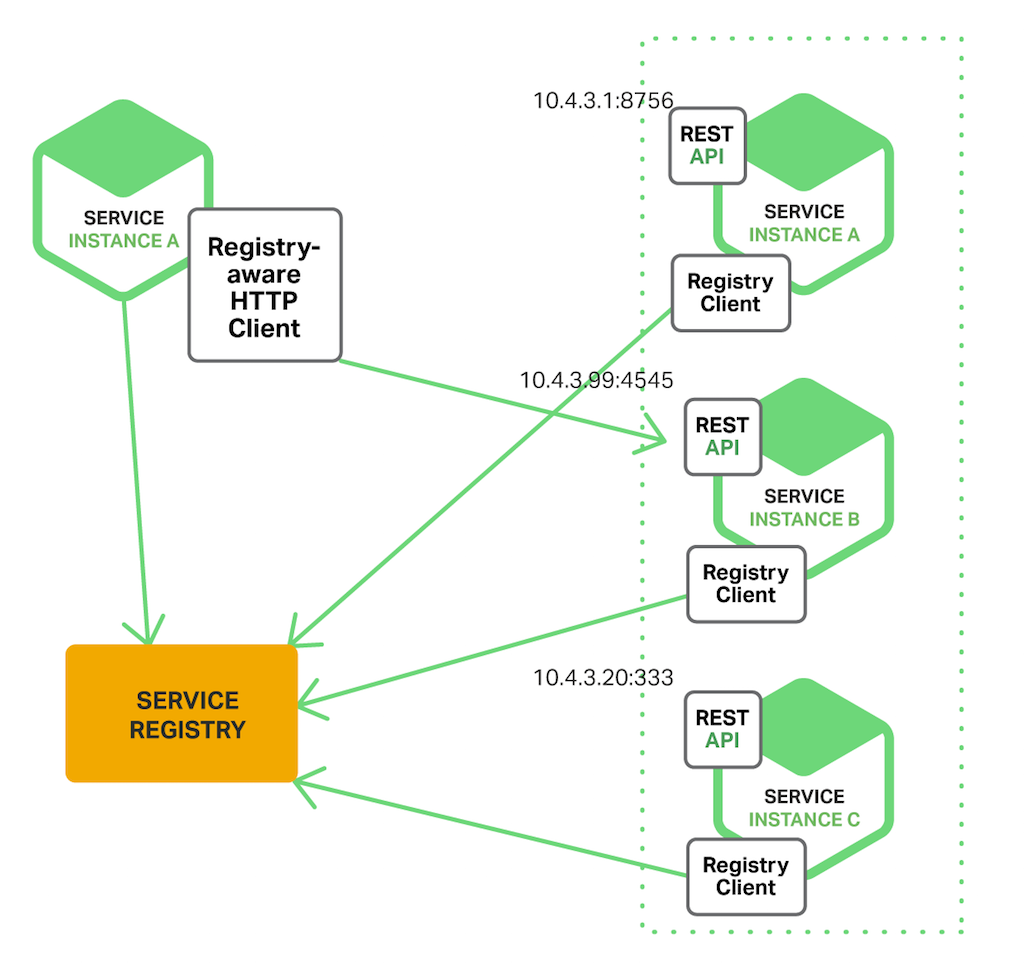
\includegraphics[scale=0.18]{img/Richardson-microservices-part4-2_client-side-pattern.png}
\caption{Identificarea serviciilor de către client}
\label{fig:arhi_componente}
\end{figure}

Acest mod de funcționare prezintă o varietate de beneficii și dezavantaje. Se bazează pe un principiu simplu și exceptând registrul serviciilor nu există alte componente mobile. În plus, din moment ce serviciul cunoaște toate instanțele de serviciu disponibile, poate să ia decizii de balansare inteligente, specifice aplicației. Un dezavantaj major este cuplarea clientului cu registrul serviciilor; în acest caz trebuie implementată o logică de descoperire a serviciilor pentru fiecare limbaj de programare și set de biblioteci folosite de către serviciile-client. 

\subsection{Identificarea serviciilor de către server}

Cealaltă abordare posibilă este identificarea serviciilor de către server, care funcționează conform schemei de mai jos:

\begin{figure}[ht]
\centering
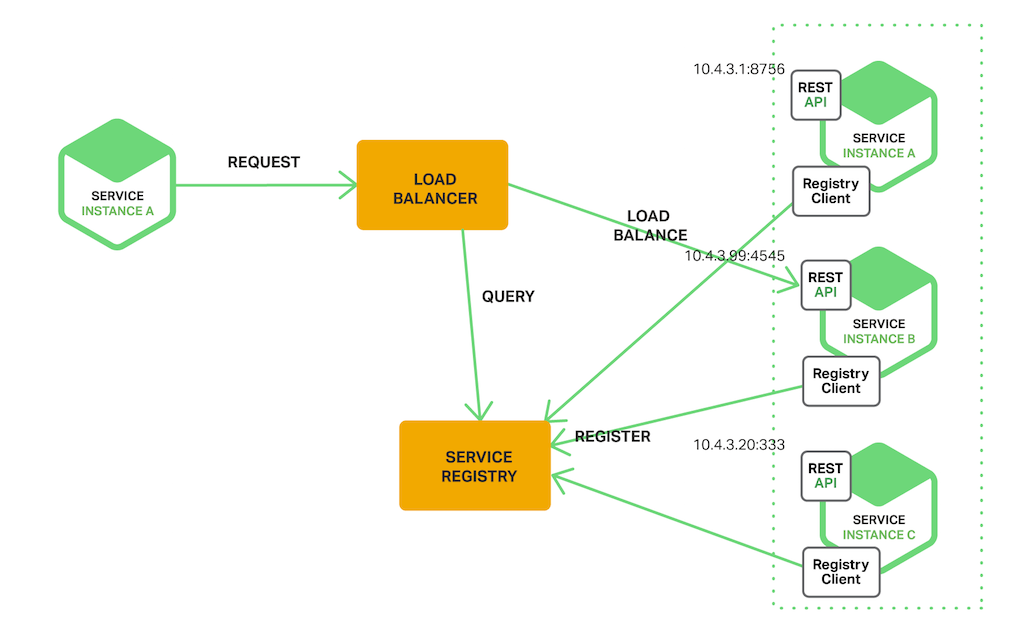
\includegraphics[scale=0.22]{img/Richardson-microservices-part4-3_server-side-pattern.png}
\caption{Identificarea serviciilor de către server}
\label{fig:arhi_componente}
\end{figure}

Clientul lansează o cerere către serviciu prin intermediul unui load balancer, care la rândul său interoghează registrul de servicii și rutează fiecare cerere către o instanță a serviciului. Ca și în cazul identificării de către client, instanțele de serviciu sunt gestionate de registrul de servicii. 

AWS Elastic Load Balancer (ELB), produs al companiei Amazon este un exemplu de asemenea mecanism. Este folosit în principiu pentru a balansa traficul extern venit din Internet. Totuși poate fi folosit pentru a distribui traficul care este intern unui cloud privat. Un client lansează cereri via ELB folosind numele DNS. Acesta distribui traficul între instanțele înregistrate. Nu există un registru de servicii separat, în schimb toate aceste instanțe sunt înregistrate direct în ELB.

Unele medii care folosesc Kubernetes sau Marathon folosesc un proxy la nivelul fiecărei mașini din cluster. Proxy-ul joacă rolul load-balancer-ului responsabil pentru descoperire de către server. Pentru a lansa o cerere către un serviciu, un client rutează cererea via proxy folosind adresa IP a hostului și portul serviciului. Apoi proxy-ul transmite mai departe cererea către o instanță disponibilă din cluster.

Acest mod de funcționare prezintă deasemenea avantaje și dezavantaje. Un mare avantaj ar fi faptul că detaliile legate de identificare sunt decuplate de client. Aceștia lansează pur si simplu cereri către load balancer, ceea ce elimină nevoia implementării unei logici de identificare pentru fiecare limbaj de programare sau set de biblioteci folosit de către serviciile client. Există totuși și dezavantaje. Dacă funcționalitatea nu este livrată împreună cu mediul de instalare, este încă o componente ce trebuie configurată și menținută. 

\subsection{Registrul serviciilor}
Registrul serviciilor este o parte cheie din procesul de identificare a serviciilor. Este o bază de date ce conține locațiile de rețea ale instanțelor serviciilor. Acesta trebuie să fie o componentă cu un grad înalte de disponibilitate și mereu actualizat. Clienți pot stoca în memoria cache locațiile de rețea obținute de la acesta, însă informația va deveni la un moment dat învechită și clienții vor fi nevoiți să reapeleze registrul. În consecință, un regitru de servicii reprezintă un cluster de server care folosesc un protocol de replicare pentru a menține consistența.

Un exemplu de astfel de componentă este Eureka. Acesta oferă un API de tip REST pentru înregistrarea instanțelor de serviciu, cât și pentru interogări. O instanță de serviciu se înregistrează printr-o cerere de tip POST. La fiecare 30 de secunde înregistrarea trebuie actualizată printr-o cerere de tip PUT. Înregistrarea este ștearsă fie folosind o cerere HTTP DELETE fie pentru expirarea unui timer. Un client poate obține lista de instanțe înregistrate folosind o cerere de tip HTTP GET.

Alte exemplu de astfel de componente:

\begin{itemize}
 \item \textbf{etcd} - reprezintă o componentă de stocare de tip cheie-valoare cu un grad înalte de disponibilitate folosit pentru stocarea configurațiilor și pentru identificarea serviciilor. Două proiecte notabile care folosesc această componentă sunt Kubernetes și Cloud Foundry. 
 \item \textbf{consul} - este o unealtă pentru identificarea și configurarea serviciilor. Oferă un API care permite clienților să se înregistreze și să descopere servicii. Acesta poate efectua verificări pentru determinarea disponibilității serviciului. 
 \item \textbf{Apache Zookeeper} - este un serviciu de coordonare a aplicațiilor distribuite foarte răspândit. Inițial a fost un subproiect Hadoop, dar acum a devenit un proiect separat. 
\end{itemize}

Deasemenea, este de notat faptul ca sisteme pentru Kubernetes, Marathon și AWS nu au un registru al serviciilor explicit. În schimb, acesta este o componentă integrată a infrastructurii.

\newpage
\subsection{Metode de înregistrare a serviciilor}

Așa cum am menționat anterior, instanțele de serviciu trebuie să fie înregistrare și șterse din registrul serviciilor. Există câteva modalități pentru a gestiona aceste două operațiuni. Una este ca serviciile să se înregistreze ele însele, numit și auto-înregistrare. Cealaltă opțiune este ca o componentă a sistemului să gestioneze aceast, numit și înregistrare terță.

\subsubsection{Auto-înregistrarea}
Folosind auto-înregistrarea, o instanță a serviciului este reponsabilă pentru înregistrare și anularea acesteia din cadrul registrului. Deasemenea, dacă este necesar, instanța serviciului trimite pulsuri pentru a preveni expirarea înregistrării.

\begin{figure}[ht]
\centering
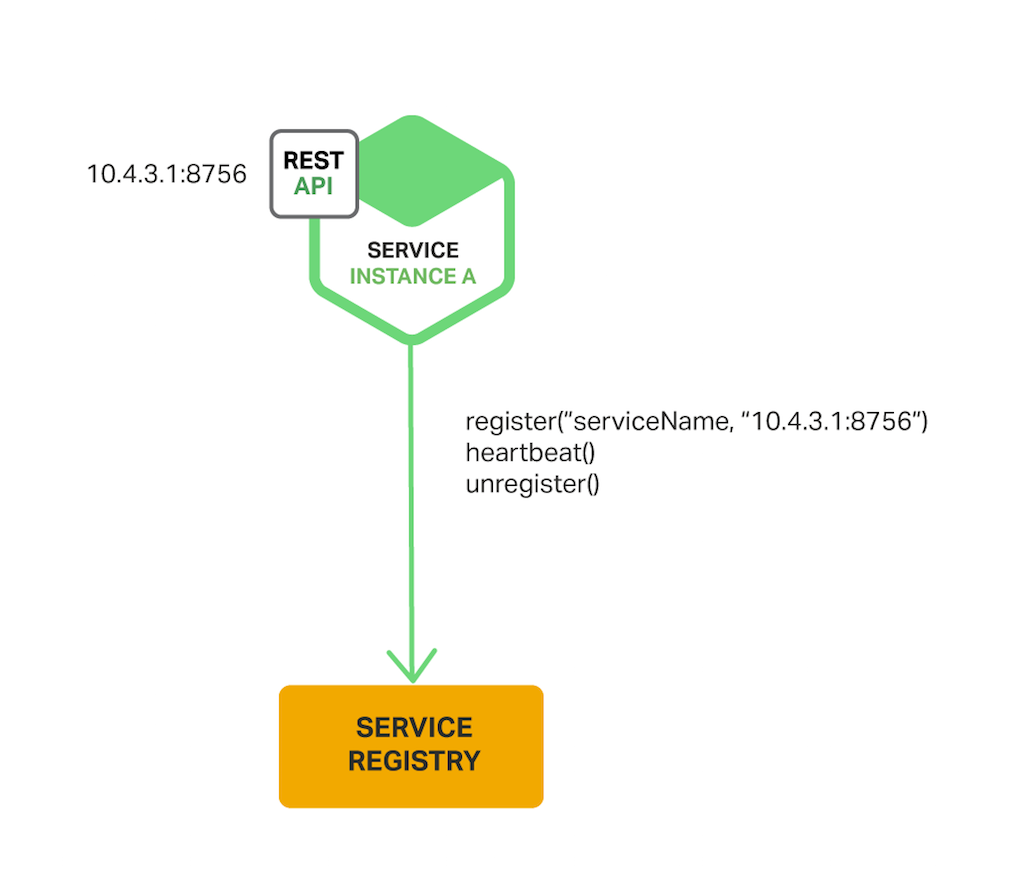
\includegraphics[scale=0.22]{img/Richardson-microservices-part4-4_self-registration-pattern.png}
\caption{Auto-înregistrare}
\label{fig:arhi_componente}
\end{figure}

Un exemplu bun al acestei abordări este client Eureka. Acesta se ocupă de toate aspectele legate de înregistrarea și înlăturarea unei instanțe în registrul serviciilor. Proiectul Spring Cloud, care implementează o serie de șabloane încluzând identificarea serviciilor, facilitează abonarea unui serviciu la Eureka printr-o simplă anotare \texttt{@EnableEurekaClient}.

Un prim avantaj al acestei metode ar fi simplitatea, datorită faptului că nu necesită nici o altă componentă de sistem. Însă, dezavantajul major este cuplarea între instanțe și registrul serviciilor. Aceasta crează necesitatea codării acestei funcționalităti la nivelul fiecărui limbaj de programare.

Abordarea alternativă, care decuplează serviciile de registrul serviciilor, este înregistrarea terță.
\newpage
\subsubsection{Înregistrarea terță}
Folosind înregistrarea terță, instanțele serviciuliu nu mai sunt responsabile pentru înregistrarea în cadrul registrului serviciilor. În schimb, o altă componentă de sistem cunoscută sub numele de registrar al serviciilor (\textit{eng. service registrar}) se ocupă de aceasta. Acesta monitorizează schimbările la nivelul instanțelor fie prin interogări periodice al mediului de instalare fie prin abonarea la evenimente. Atunci când detectează o nouă instanță acesta o înregistrează la nivelul registrului. Deasemenea tot el se va ocupa și de eliminare înregistrării în momentul în care instanța nu mai este  disponibilă. 

\begin{figure}[ht]
\centering
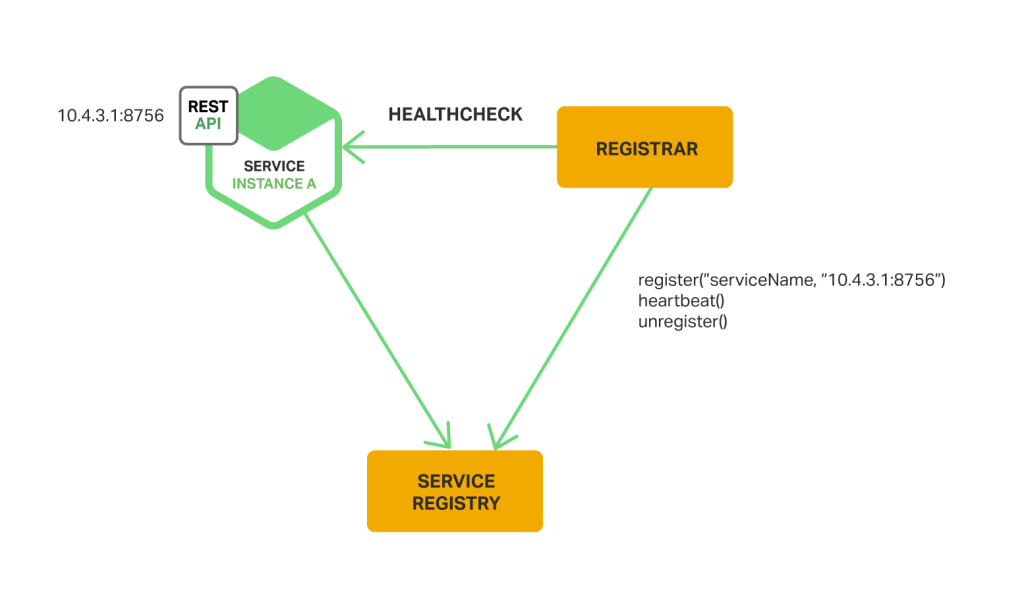
\includegraphics[scale=0.3]{img/Richardson-microservices-part4-5_third-party-pattern.png}
\caption{Înregistrare terță}
\label{fig:arhi_componente}
\end{figure}

Un exemplu de o astfe de componentă este proiectul open-source Registrator. Acesta este capabil să gestioneze instanțele de serviciu care sunt instalate ca și containere Docker. Acesta dispune suport pentru o serie de registrii de servicii precum, \texttt{etcd} și \texttt{Consul}.

Principalul beneficiu al acestui mod de funcționare este faptul că decuplează serviciile de registrul serviciilor. Nu mai este necesară implementarea logici la nivelul fiecărui limbaj de programare, în schimb procesul este gestionat într-o manieră centralizată de către un serviciu dedicat. Dezavantajul este că, dacă nu este furnizat de mediul de instalarea acesta devine încă o componentă ce trebuie configurată și menținută. 


\end{document}